\documentclass{beamer}
\usepackage[utf8]{inputenc}
\usepackage{graphicx}
\usepackage{color}
%\usetheme{Hannover}
\newcommand{\hilight}[1]{\textbf{\textcolor{structure.fg!85}{#1}}}
\setbeamertemplate{footline}[frame number]
\setbeamertemplate{footline}[frame number]

\usepackage{hyperref}
\hypersetup{
    colorlinks=true,
    linkcolor=blue,
    filecolor=magenta,      
    urlcolor=cyan,
}

\author[Sowmya Vajjala]{Sowmya Vajjala}

\title[SfSNLP]{NLP without Annotated Dataset}
\subtitle{NLP Pipeline and Text Representation}
%: \\ on using insights from language acquisition, cognitive science and psychology research

\date{11 January 2021}

\institute{Seminar f\"ur Sprachwissenschaft, University of T\"ubingen, Germany}
%%%%%%%%%%%%%%%%%%%%%%%%%%%

\begin{document}

\begin{frame}\titlepage
\end{frame}

\begin{frame}
\frametitle{Class Outline}
\begin{itemize}
    \item Quick recap of last class
    \item How do we build NLP systems?
    \item A typical NLP Pipeline
    \item Case study of a real-world NLP pipeline
    \item Building an NLP Pipeline - an example
    \item Sharing some personal experiences from an industry project.
    \item Feature Engineering- How do we represent text for NLP?
\end{itemize}
As per student suggestions, let us take a 5 min break each at about 45 min, and at about 1.5 hrs.
\end{frame}

\begin{frame}
\frametitle{Last Class: Quick Recap}
\begin{itemize}
    \item What is NLP, where is it useful?
    \item Why is NLP difficult?
    \item Some common NLP tasks
    \item levels of language processing
    \item NLP methods
\end{itemize}
- Any questions on anything from the last class or about the course so far?

\end{frame}

\begin{frame}
\frametitle{General Housekeeping}
\begin{itemize}
    \item New zoom room
    \item Messages about teams, termpapers etc.
    \item Participation in forums ( and new forums)
    \item Breaks in between from now on (2 5 min breaks)
    \item Today's class also hopefully has more interaction/questions to you
    \item Some extra stuff ( text representation) in slides today 
\end{itemize}
\end{frame}

\begin{frame}
\frametitle{What does NLP involve?}
\begin{itemize}
    \item Some basic linguistic ideas (e.g., words, morphology, part of speech, syntax etc. )
    \item Different tasks (e.g., POS tagging, parsing, coreference resolution, information extraction etc)
    \item Different applications (e.g., Machine Translation, Chatbots, Question Answering etc.)
        \item Many algorithms (e.g., naive bayes, HMMs, LSTMs, Transformers etc)
\end{itemize}
How do these come together when you build an NLP system for some industry use case?
\end{frame}

\begin{frame}[fragile]
\frametitle{Option 1: Utilize Existing Services}

We don't always have to build everything ourselves. We can use a pay as you go service from a third party provider. 

\newline An example: Microsoft's machine translation API
\tiny
\begin{verbatim}
import os, requests, uuid, json
subscription_key = "XXXX"
endpoint = "https://api-nam.cognitive.microsofttranslator.com"
path = '/translate?api-version=3.0'
params = '&to=de' #From English to German (de)
constructed_url = endpoint + path + params
headers = {
    'Ocp-Apim-Subscription-Key': subscription_key,
    'Content-type': 'application/json',
    'X-ClientTraceId': str(uuid.uuid4())
}

body = [{'text' : 'How good is Machine Translation?'}]
request = requests.post(constructed_url, headers=headers, json=body)
response = request.json()

print(json.dumps(response, sort_keys=True, indent=4, separators=(',', ': ')))
\end{verbatim}
source: \href{https://github.com/practical-nlp/practical-nlp/blob/master/Ch7/05_MachineTranslation.ipynb}{Practical NLP, Ch 7}
\end{frame}

\begin{frame}[fragile]
\frametitle{Output}
\small
\begin{verbatim}
[
    {
    "detectedLanguage": {
          "language": "en",
          "score": 1.0
    },
    "translations": [
          {
               "text": "Wie gut ist maschinelle Übersetzung?",
               "to": "de"
          }
    ]
    }
]
\end{verbatim}
\end{frame}

\begin{frame}
\frametitle{Advantages and Disadvantages}
\begin{itemize}
    \item Advantage: You don't have to worry about setting stuff up,  hiring a large NLP team, maintaining the NLP system etc. 
    \item Disadvantages:
    \begin{enumerate}
        \item This only works if you have problem that exactly meets the specifications of such an available API
        \item No possibility of customization/modification  
        \item Depending on how much you use, costs may escalate
    \end{enumerate}
    Note: You still have to think whether this approach is a long term solution for your problem.
\end{itemize}
\end{frame}

\begin{frame}
\frametitle{Short Exercise}
\begin{itemize}
    \item Spend 5 minutes on the internet and look for NLP services from Cloud providers such as Google, Microsoft, Amazon, Watson etc.
    \item Make a note of what sort of services do they provide for NLP applications. 
\end{itemize}
\end{frame}

\begin{frame}
\frametitle{What is more likely to happen, though?}
\begin{itemize}
    \item Say you have custom problem (e.g., classify customer tweets about your product into "actionable" and "non-actionable" ones. )
    \item Will any of these off the shelf solutions work? \pause
    \item What do we need to design a solution for this problem?? \pause
    \item First of all, we need "data". What Data? for what? \pause
    \begin{enumerate}
        \item To "train" NLP models
        \item To "evaluate" and validate NLP models
    \end{enumerate}
    \pause \item ... and then?
\end{itemize}
\end{frame}

\begin{frame}
\frametitle{NLP System Development Pipeline}
\framesubtitle{A Common Case}
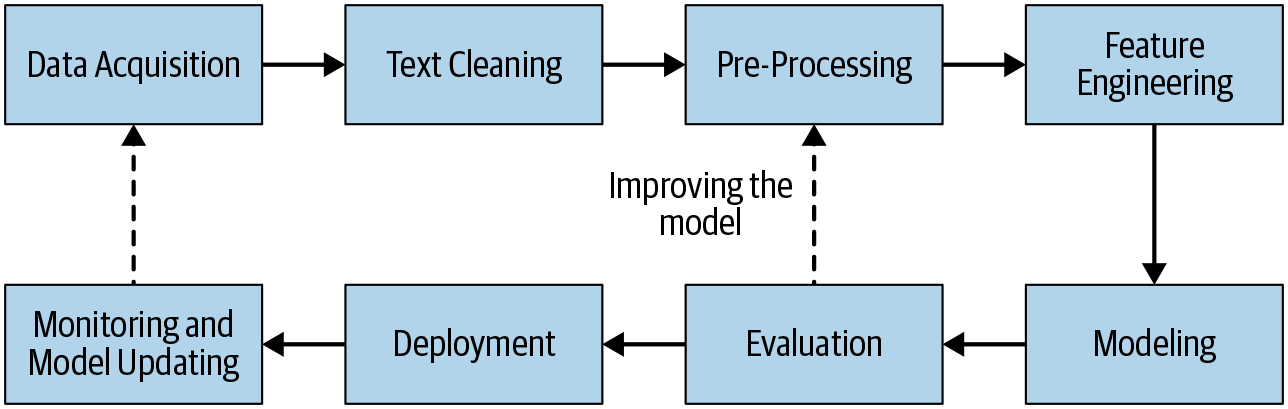
\includegraphics[width=\textwidth]{figures/pipeline.png}
\end{frame}

\begin{frame}
\frametitle{Data Acquisition}
\begin{itemize}
    \item Where do we get our data from? \pause
    \item Let us say you are working in a software company, and they asked you to develop a customer ticket routing system that looks at a ticket text, and classifies it into three categories: technical, sales, other. Where will your data come from?
    \pause \item In an ideal scenario, we have some historical data of customer tickets along with this routing information.
    \item But what if they were just routing to the right team, but not storing that information anywhere in the past? We don't have the training data we want!
\end{itemize}
\end{frame}

\begin{frame}
\frametitle{How do we get our Data?}
\begin{itemize}
    \item use a public NLP dataset (e.g., https://datasets.quantumstat.com/) \pause
    \item scrape the data from the web (e.g., customer support forums of other products, if they are available and are tagged with categories)
    \item work together with your customer support team and gradually collect the data you want. 
    \item using pattern matching and other such methods to create some data to train your own models and gradually improve this baseline. 
    \item setting up data annotation experiments
\end{itemize}
.... and so on. 
\end{frame}

\begin{frame}
\frametitle{Text Extraction and Cleaning}
\begin{itemize}
    \item What, according to you, is the format of data you see in NLP? \pause
    \item Data can come in all forms: PDF, Docs, HTML files, scanned png files, tables etc.
     \item Text extraction and cleanup refers to the process of extracting raw text from the input data by removing all the other non-textual information.
     \item Text extraction may not involve NLP per se, but it defines the rest of your NLP pipeline. Bad text extraction = Bad NLP system.
\end{itemize}
\end{frame}

\begin{frame}
\frametitle{Text Extraction: Some facts}
\begin{itemize}
    \item PDF to text conversion is hard and imperfect. Not all pdfs can be efficiently parsed. \pause
    \item When we are extracting text from images, We may see some characters not rendered properly, or some words extracted with spelling mistakes etc
    \item If all of the "dataset" is a large collection of pdf documents with scanned text along with some tables: it is like the worst of all NLP worlds  :-) 
    \item We don't have a single solution that works for all. There are tools like Amazon Textract, but they are not perfect. 
\end{itemize}
\end{frame}

\begin{frame}
\frametitle{Text Pre-processing}
\begin{itemize}
    \item Sentence segmentation and word tokenization \pause
    \item Stop word removal, stemming and lemmatization, removing digits/punctuation, lowercasing, etc. \pause
    \item Normalization, language detection, code mixing, transliteration, etc. \pause
    \item POS tagging, parsing, coreference resolution, etc.
\end{itemize}
(you probably are already familiar with some of these.)
\end{frame}

\begin{frame}
    \Large Questions so far?
\end{frame}

\begin{frame}
\frametitle{Feature Engineering}
\begin{itemize}
    \item The goal of feature engineering is to capture the characteristics of the text into a numeric vector that can be understood by the ML algorithms.
    \item There are primarily two ways of feature extraction in NLP:
    \begin{enumerate}
        \item  hand crafted features (e.g., number of words/sentences in a document, number of spelling errors/sentence etc.)
        \item automatically extracted features (e.g., Bag of words, Bag of N-grams etc.)
    \end{enumerate}
\end{itemize}
\end{frame}

\begin{frame}
\frametitle{Modeling}
\begin{itemize}
    \item Heuristics based systems (e.g., regular expressions, rule based matching etc)
    \item Learning from data: Machine learning (e.g., logistic regression, support vector machines etc.), deep learning
\item Model ensemble (combining predictions from multiple models)
\item Model cascade (using one model's prediction as input to another model)
\end{itemize}
.......
\end{frame}

\begin{frame}
\frametitle{Evaluation}
How well is my NLP approach doing?
\begin{itemize}
    \item Intrinsic evaluation focuses on intermediary objectives, while extrinsic focuses on evaluating performance on the final objective. \pause
    \item Consider a email spam classification system:
  \begin{enumerate}
      \item Intrinsic evaluation will focus on measuring the system performance using precision and recall. 
      \pause \item Extrinsic evaluation will focus on measuring the time a user wasted because a spam email went to their inbox or a genuine email went to their spam folder.
  \end{enumerate}
\end{itemize}
\end{frame}

\begin{frame}
\frametitle{Deployment, Monitoring and Model Updating}
\begin{itemize}
    \item Once we have a good model, we have to deploy it in the context of a larger system (e.g., spam classification is a part of an email software)
\item A common approach: deploy the NLP system as a micro service/web service
\item Model monitoring: e.g., using a performance dashboard showing the model parameters and key performance indicators
\item Model updating: Model has to stay current, with changing data. So, we should have some way of regularly updating, evaluating and deploying a model.
\end{itemize}
\end{frame}

\begin{frame}
\frametitle{Pipeline Variation: Deep Learning Pipeline}
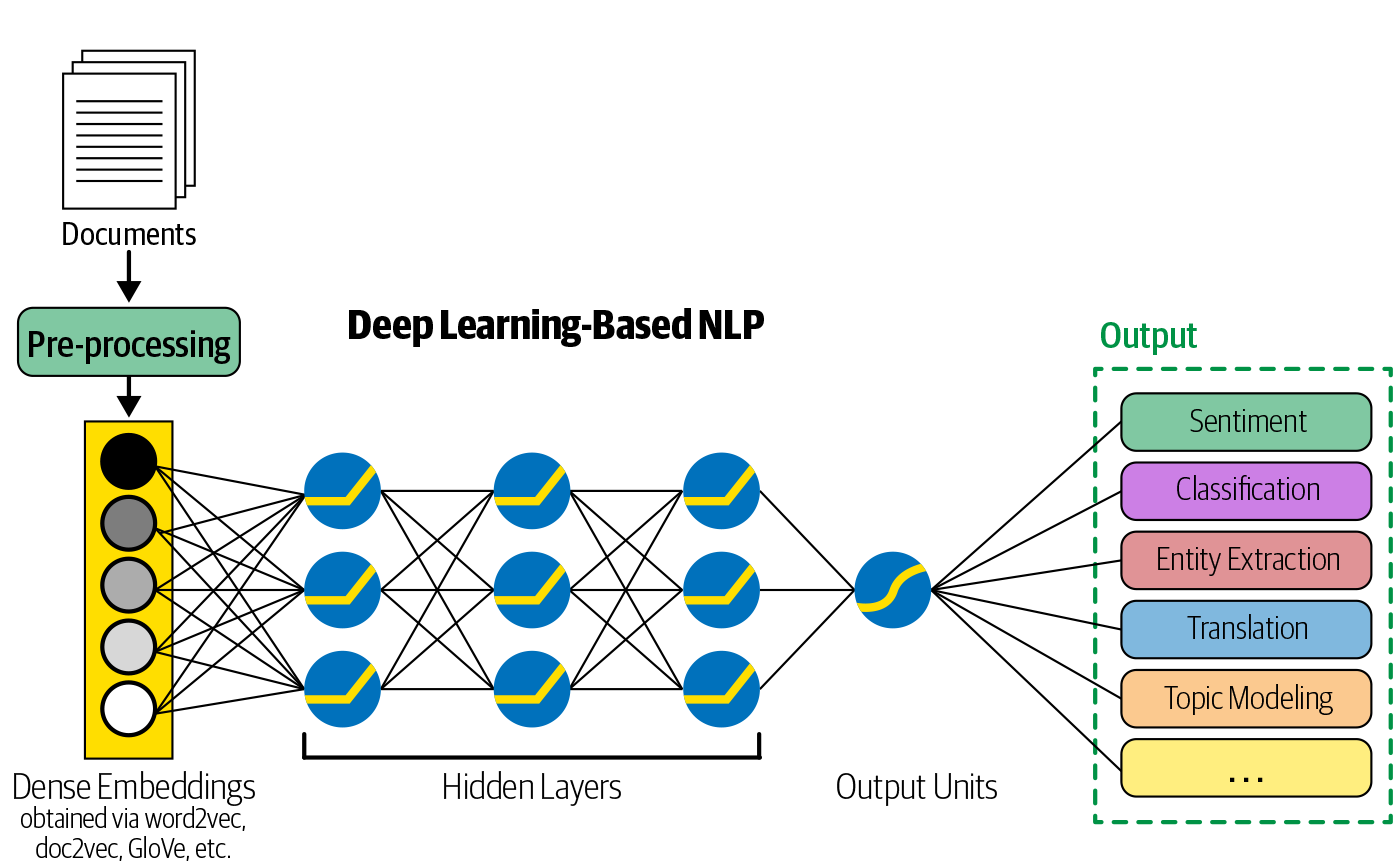
\includegraphics[width=\textwidth]{figures/nlppipelinedl.png}
[source](https://blog.aylien.com/leveraging-deep-learning-for-multilingual/)
\end{frame}


\begin{frame}
\frametitle{Pipeline Variation: Transfer Learning Pipeline}
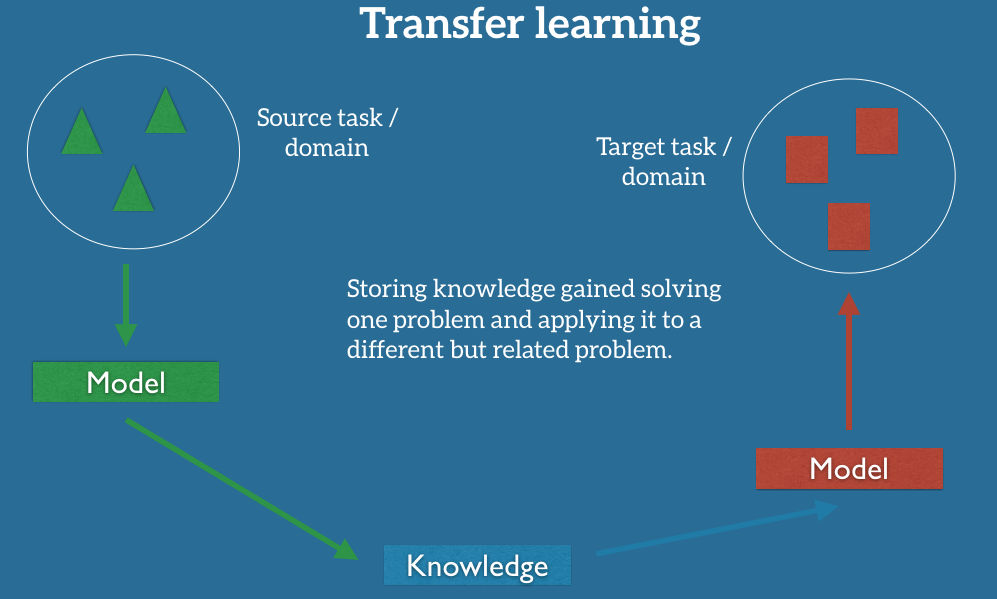
\includegraphics[width=\textwidth]{figures/tl.png}
[source](https://ruder.io/transfer-learning/)
\end{frame}

\begin{frame}
\frametitle{NLP Pipeline: Some Questions}
\begin{itemize}
    \item What is the difference between traditional pipeline and deep learning pipeline?
\item What are some advantages and disadvantages of deep learning?
\item What are some advantages and disadvantages of transfer learning? 
\item If you already know some ML/deep learning usage, how many steps of this pipeline did you learn/think about so far? 
\end{itemize}
\end{frame}

\begin{frame}
\frametitle{Pipeline Variation: Automated ML}
\begin{itemize}
    \item Automated ML is the process of automating the process of building machine learning based systems (provided you have your data in place) so that even those with minimal ML knowledge can also use it.
    \item The goal is to automate the iterative process of training/testing multiple models, parameter settings etc.
    \item Google, Microsoft etc provide AutoML options for various tasks. 
\end{itemize}
\end{frame}

\begin{frame}
\frametitle{Advantages and Disadvantages}
Advantages:
\begin{itemize}
    \item We don't need an expert machine learning or NLP team
    \item We don't have to worry about training/tuning the model well
    \item We can get by with writing minimum "machine learning" related code ourselves.
\end{itemize}
Disadvantages:
\begin{itemize}
    \item This works only if we have a large amount of training data already in place.
    \item It is still hard to customize if we have some custom pre/post processing, feature engineering etc. 
\end{itemize}
\end{frame}

\begin{frame}
\frametitle{Short Exercise}
\begin{itemize}
    \item Spend 5 minutes on the internet and look for what AutoML feature of Google and Microsoft looks like. 
\end{itemize}
\end{frame}

\begin{frame}
\frametitle{A real-world NLP pipeline: Uber's COTA}
\begin{itemize}
    \item It is a tool used within Uber to help agents do better customer support, by supporting quick and efficient issue resolution for a majority of Uber's support tickets. 
\item (i.e., instead of asking the customer to answer several questions related to the issue, automate that process so that agents can react more quickly.) \pause
\item Task: identify the issue type, and find out the right resolution based on ticket text, and other info such as trip data. 
\end{itemize}
"COTA can reduce ticket resolution time by over 10 percent while delivering service with similar or higher levels of customer satisfaction"
\end{frame}

\begin{frame}
\frametitle{Uber COTA V1}
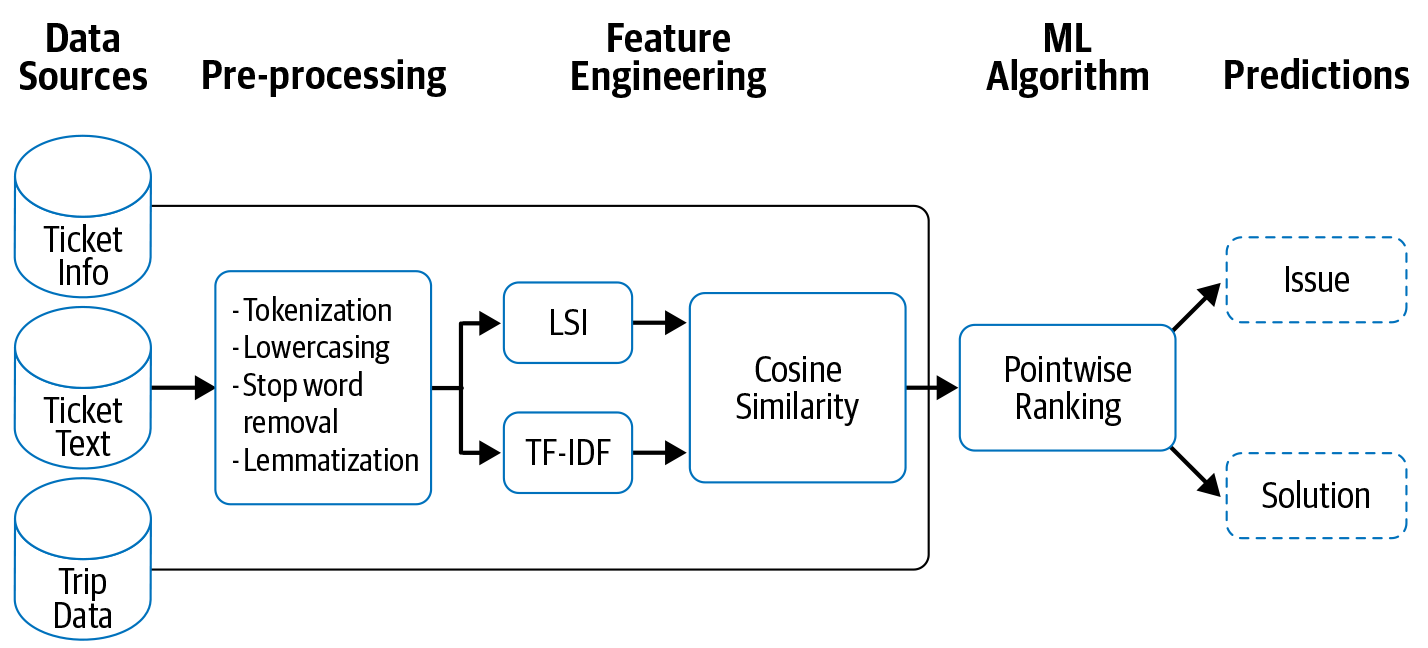
\includegraphics[width=\textwidth]{figures/nlpcaseuber.png}
[source](https://eng.uber.com/cota/)
\end{frame}


\begin{frame}
\frametitle{Uber COTA V2: A Deep Learning Pipeline}
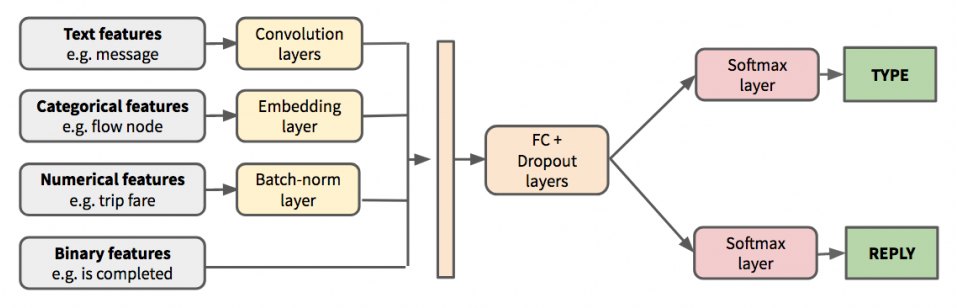
\includegraphics[width=\textwidth]{figures/cotav2.png}
[source](https://eng.uber.com/cota-v2//)
\end{frame}

\begin{frame}
\frametitle{NLP Pipeline: Some Questions}
\begin{itemize}
    \item What is one important thing you learnt from this quick look at COTA?
 \pause \item For me, it is: 
 \begin{enumerate}
     \item start with a relatively straight forward approach, and build incrementally.
     \item We don't have to start with deep learning.  
     \item Have your extrinsic evaluation measures in place (here: speed of resolution or improved customer support experience etc) along with intrinsic ones
 \end{enumerate}
\end{itemize}
\end{frame}

\begin{frame}
\frametitle{Few More Questions}
\begin{itemize}
    \item What according to you is the most important part of the NLP Pipeline? \pause
    \item Should our data to train an NLP system come from only a single source?  \pause
    \item When are rule based "models" relevant? 
    \item What can be a rule based approach to developing a sentiment analyzer?
\end{itemize}
\end{frame}

\begin{frame}
\frametitle{A code Example: Sentiment Analyzer}
\begin{itemize}
    \item 
\end{itemize}
source code for \href{https://github.com/nlpwithoutdataset/MBDS2018-NLPTutorial/blob/master/code/TextClassificationSKLearn.py}{Training} and \href{https://github.com/nlpwithoutdataset/MBDS2018-NLPTutorial/blob/master/code/SentimentClassifier.py}{Using a model}
\end{frame}

\begin{frame}[fragile]
\frametitle{Text Extraction and Pre-processing}
\tiny
\begin{verbatim}
#Read the training file and do the required pre-processing
def getData(file_path):
    #col1: Move cat. #last col: Text
    fh = open(file_path)
    texts = []
    cats = []
    fh.readline() #Header
    for line in fh:
        temp = line.split(",")
        text = " ".join(temp[1:])
        texts.append(" ".join(removepunct_tokenize_stem(text)))
        cats.append(temp[0])
    fh.close()
    return texts,cats
\end{verbatim}
\end{frame}

\begin{frame}[fragile]
\frametitle{Text Extraction and Pre-processing}
\framesubtitle{pre-processing}
\tiny
\begin{verbatim}
#Stemming. Optional.
def stem_tokens(tokens, stemmer):
    stemmed = []
    for item in tokens:
        stemmed.append(stemmer.stem(item))
    return stemmed

#Remove punctuation, and perform stemming - again, optional. Just a choice I made.
#You can build a classifier without doing these - it will work, may be not as efficiently.
def removepunct_tokenize_stem(text):
    text = "".join([ch for ch in text if ch not in string.punctuation]) #Remove punctuation
    tokens = word_tokenize(text)
    stemmer = PorterStemmer()
    final = stem_tokens(tokens, stemmer)
    return finals
\end{verbatim}
\end{frame}

\begin{frame}[fragile]
\frametitle{Feature Engineering and Model Building}
\tiny
\begin{verbatim}
#Learns a classifier with the specified features in CountVectorizer 
#and saves the model so that we can use it again to make predictions
def save_model(texts,cats,model_file):
    vectorizer =  CountVectorizer(analyzer = "word", tokenizer = None, 
                  preprocessor = None, stop_words = None, ngram_range=(1,2), min_df=10)
   # classifier =  LinearSVC(max_iter=500)
    classifier = LogisticRegression(max_iter=100,class_weight="balanced",random_state=1234)
    pipeline = Pipeline([('vectorizer', vectorizer), ('pac', classifier)])
    pipeline.fit(texts,cats)
    joblib.dump(pipeline, model_file)
    print("Model saved as: ", model_file)
\end{verbatim}
\end{frame}

\begin{frame}{Notes}
We normally explore: 
    \begin{itemize}
    \item multiple vectorization methods (single words, characters, word ngrams etc), multiple settings within one method (e.g., top 1000 features, top 5000, with or without certain pre-processing etc) (More on this at the end of today's class)
    \item multiple training approaches (e.g., logistic regression, decision trees etc) and different parameter settings (e.g., number of training iterations, any other tunable parametres etc)
    \item various evaluation measures (e.g., accuracy, F1 score, precision, recall etc)
    \end{itemize}
... to build many different models and choose the best one, and save that one. 
\end{frame}

\begin{frame}[fragile]
\frametitle{Using the Classifier}
\tiny
\begin{verbatim}
#Makes prediction for a single string.
def makePredictionsForAString(inputstr,classifier):
    converted = [" ".join(removepunct_tokenize_stem(inputstr))]
    all_predictions = list(classifier.predict_proba(converted)[0])
    predict_prob = max(all_predictions)
    print(predict_prob)
    prediction = classifier.predict(converted)[0]
    print(inputstr[:50]+"...", prediction)

\end{verbatim}
\end{frame}

\begin{frame}
\frametitle{NLP Pipeline: A Personal Experience}
Scenario: NER for legal documents (e.g., agreements etc) which are PDFs. \pause

Our options:
\begin{itemize}
\item use an off the shelf solution, tune it to your domain, and then deploy \pause
\item build your own NER model, using rules \pause
\item build your own NER using machine learning/deep learning
\end{itemize}
\end{frame}

\begin{frame}[fragile]
    \frametitle{Off the shelf NER}
\tiny
\begin{verbatim}
import spacy
nlp = spacy.load("en_core_web_sm")
doc = nlp("Apple is looking at buying U.K. startup for $1 billion")

for ent in doc.ents:
    print(ent.text, ent.start_char, ent.end_char, ent.label_)
    
Output: 
Apple 0 5 ORG
U.K. 27 31 GPE
$1 billion 44 54 MONEY
\end{verbatim}
\end{frame}

\begin{frame}
\frametitle{off the shelf NER + Adapt to your domain}
using "active learning": annotate examples that the model does not know yet, and the model adapts, as it sees them.
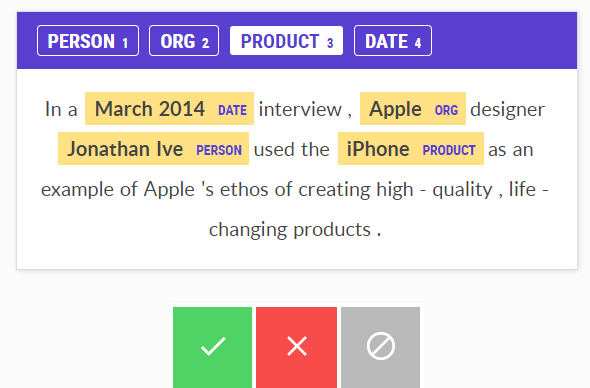
\includegraphics[width=0.9\textwidth]{figures/prodigy.png}

\tiny \url{https://prodi.gy/docs/named-entity-recognition}
\end{frame}

\begin{frame}
\frametitle{Build your own NER Model using rules}
\begin{itemize}
\item a lookup table with a large collection of names of people/organizations/etc relevant for your organization \pause
\item a bunch of hand crafted rules (e.g., a proper noun followed by "was born" may indicate a person) etc.
\end{itemize}
Spacy's \href{https://spacy.io/usage/rule-based-matching#entityruler}{Entity Ruler} is a useful tool for this kind of an approach. 
\end{frame}

\begin{frame}{Build your own NER model using machine/deep learning}
\begin{itemize}
    \item \href{https://github.com/practical-nlp/practical-nlp/blob/master/Ch5/02_NERTraining.ipynb}{using feature engineering + machine learning}
    \item \href{https://github.com/practical-nlp/practical-nlp/blob/master/Ch5/04_NER_using_spaCy - CoNLL.ipynb}{using spacy's training pipeline (deep learning)}
    \item \href{https://github.com/practical-nlp/practical-nlp/blob/master/Ch5/05_BERT_CONLL_NER.ipynb}{using transfer learning}
\end{itemize} 
\end{frame}

\begin{frame}{What we did}
    \begin{itemize}
        \item Explored various NLP libraries and cloud providers. We figured they don't do so well for our use case.
        \item Trained our own NER with a standard dataset (CONLL-03), and with simple features, as a base NER model.
        \item Used prodi.gy for domain specific annotation, and added these examples to the existing model to update it (and tune it for legal docs)
        \item Added some rules/heuristics on top of a machine learning model
        \item Explored a model ensemble with 2-3 models
        \item Looked at training with noisy text (i.e., output of pdf to text conversion + sentence/word segmentation)
    \end{itemize}
    ... ... 
\end{frame}

\begin{frame}{Some Observations}
    \begin{itemize}
        \item off the shelf NER is not perfect, but it is a good starting point.
 \item If you have only a small amount of annotated data for your domain, you can explore transfer learning, and gradually collect more domain specific data. 
\item A reliable approach afterwards: rules + (feature engineering + model) 
\item If you want to use deep learning, check if it is better than the above process first (for any NLP problem)
\item Remember: your implementation should also be deployable, not just accurate. 
    \end{itemize}
    ... ... 
\end{frame}

\begin{frame}{More observations}
    \begin{itemize}
        \item There is no single model. We have to set up a model monitoring/updating pipeline using some evaluation criteria. 
\item There is no single training set or test set. They will also evolve with time. \pause
\item  NLP tools we use in our pipeline are not perfect. Even a simple thing as text extraction or tokenization can have many unresolved issues. While our models are all very valuable effort, these steps are, too. \pause
\item  No model can solve the problem of data quality. So, focus on getting good quality data to solve your problem first. \pause
\item Build a solution incrementally. Don't jump into the most complex solution first. Eventually, you want your stuff to be reliable, and not too expensive to maintain in short/long term. 

    \end{itemize}
    ... ... 
\end{frame}

\begin{frame}{Summary}
    \begin{itemize} 
    \item When we read about NLP in the news/research updates, we usually see models everywhere.
    \item However, there is much more behind an NLP system
    \item I hope this session introduced some of the issues behind the scenes. 
    \end{itemize}
\end{frame}

\begin{frame}{A (not so quick) detour: Text Representation}
    In "Feature Engineering", I said:
    \begin{itemize}
    \item There are primarily two ways of feature extraction in NLP:
    \begin{enumerate}
        \item  hand crafted features (e.g., number of words/sentences in a document, number of spelling errors/sentence etc.)
        \item automatically extracted features (e.g., Bag of words, Bag of N-grams etc.)
    \end{enumerate}
    - What exactly do these mean??
\end{itemize}
\end{frame}

\begin{frame}
\frametitle{What is text representation?}
\begin{itemize}
\item Any form of data text/image/video/audio should be converted into some form of numeric representation so that it can be processed by NLP/Machine Learning algorithms later
\item In NLP, this conversion of raw text to a suitable numerical form is called text representation
\item We will use text representation and feature extraction/representation as synonyms in this course.
\end{itemize}
\end{frame}

\begin{frame}
\frametitle{How is text different from any other form of data?}
\begin{itemize}
\item How do we do feature extraction with images? An image is stored in a computer as a matrix of pixels where each cell[i,j] in the matrix represents pixel i,j of the image. This matrix representation accurately represents the complete image. \pause
\item A video can be seen as a sequence of frames/images. So, it can be represented as a sequential collection of matrices. \pause
\item Consider speech—it is transmitted as a wave. To represent it mathematically, we sample the wave and record its amplitude (height).
\end{itemize}
What about text?
\end{frame}

\begin{frame}
\frametitle{Hand crafted features to represent text}
\begin{itemize}
\item When we know the domain well, it is possible to represent text as a collection of hand crafted features.
\item e.g., when I am categorizing sentiment, I can create a list of positive words, and a list of negative words, and use the \% of positive and negative words in a document as its two dimensional text representation. 
\item Assuming we come across a new problem/dataset, and we don't know where to begin, what can we do? \pause
\item in NLP, it is common to use what I will call today as **automatic text representations**, where we don't have to explicitly encode any information. 
\end{itemize}
\end{frame}

\begin{frame}
\frametitle{Consider a Toy corpus}
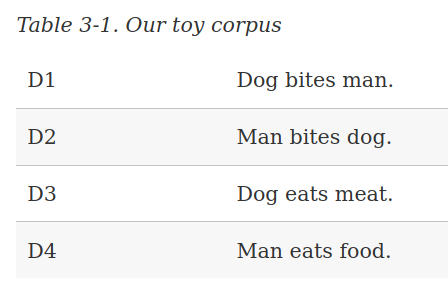
\includegraphics[width=0.9\textwidth]{figures/toycorpus.png}
\end{frame}

\begin{frame}
\frametitle{Let us start with some simple text representations}
\begin{itemize}
\item The vocabulary in this corpus, ignoring case-differences and punctuation consists of 6 words: [dog, bites, man, eats, meat, food]
\item We can organize the vocabulary in any order. In this example, we simply take the order in which the words appear in the corpus.
\item Every document in this corpus can now be represented with a vector of size six.  
\end{itemize}
\end{frame}


\begin{frame}
\frametitle{}
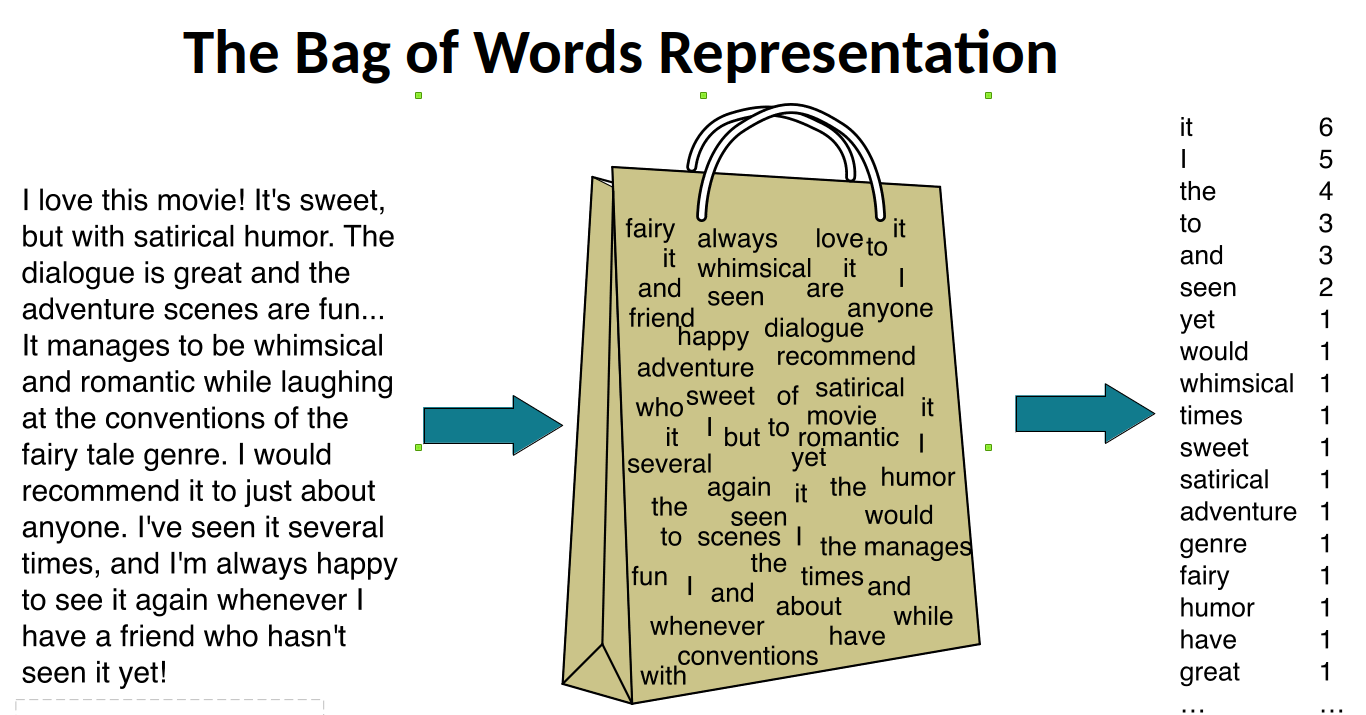
\includegraphics[width=0.9\textwidth]{figures/bow.png}
\\ \tiny source: \url{https://web.stanford.edu/~jurafsky/slp3/4.pdf}
\end{frame}

\begin{frame}
\frametitle{Bag of Words}
\begin{itemize}
\item for our toy corpus, where the word IDs are dog = 1, bites = 2, man = 3, meat = 4 , food = 5, eats = 6
\item D1 ("Dog bites man") becomes [1 1 1 0 0 0]
\item D4 ("Man eats food") becomes [0 0 1 0 1 1].
\end{itemize}
\end{frame}


\begin{frame}[fragile]
\frametitle{Code for BoW representation}
\tiny
\begin{verbatim}
from sklearn.feature_extraction.text import CountVectorizer

documents = ["Dog bites man.", "Man bites dog.", "Dog eats meat.", "Man eats food."]

#remove punctuation and lowercase words:
processed_docs = [doc.lower().replace(".","") for doc in documents]

count_vect = CountVectorizer()

#Build a BOW representation for the corpus
bow_rep = count_vect.fit_transform(processed_docs)

#Look at the vocabulary mapping
print("Our vocabulary: ", count_vect.vocabulary_)

#See the BOW rep for first 2 documents
print("BoW representation for 'dog bites man': ", bow_rep[0].toarray())
print("BoW representation for 'man bites dog: ",bow_rep[1].toarray())

#Get the representation using this vocabulary, for a new text
temp = count_vect.transform(["dog and dog are friends"])
print("Bow representation for 'dog and dog are friends':", 

temp.toarray())
\end{verbatim}
\end{frame}


\begin{frame}[fragile]
\frametitle{Bag of Words ... }
\begin{itemize}
\item If we run this code, we’ll notice that the BoW representation for a sentence like “dog and dog are friends” has a value of 2 for the dimension of the word “dog,” indicating its frequency in the text. \pause
\item Sometimes, we don’t care about the frequency of occurrence of words in text and we only want to represent whether a word exists in the text or not. Researchers have shown that such a representation without considering frequency is useful for sentiment analysis. \pause
\item In such cases, we just initialize CountVectorizer with the binary=True option keeping everything else the same. 
\begin{verbatim}
count_vect = CountVectorizer(binary=True)
\end{verbatim}
\item This results in a different representation for the same sentence. \pause
\end{itemize}
\end{frame}

\begin{frame}
\frametitle{Advantages of BoW}
\begin{itemize}
\item BoW is fairly simple to understand and implement.
\item Documents sharing vocabulary have their vector representations closer to each other in Euclidean space. In our toy corpus, distance between D1 and D2 is 0 as compared to the distance between D1 and D4, which is 2.  
\item We have a fixed-length representation for any sentence of arbitrary length.
\end{itemize}
\end{frame}

\begin{frame}
\frametitle{Disadvantages of BoW}
\begin{itemize}
\item The size of the vector increases with the size of the vocabulary. One way to control this is to take the first N most frequent words in the entire corpus.
\item t does not capture the similarity between different words that mean the same thing. Say we have three documents: “I run”, “I ran”, and “I ate”. BoW vectors of all three documents will be equally apart.
\item This representation does not have any way to handle out of vocabulary words (i.e., new words that were not seen in the corpus that was used to build the vectorizer).
\item it is a “bag” of words—word order information is lost in this representation.  Both D1 and D2 will have the same representation in this scheme.
\end{itemize}
\end{frame}

\begin{frame}
\frametitle{Bag of N-grams}
\begin{itemize}
\item BoN breaking text into chunks of n contiguous words (or tokens) called n-grams, instead of individual words 
\item This can help us capture some context,  
\item The corpus vocabulary, V, is then nothing but a collection of all unique n-grams across the text corpus. 
\item Then, each document in the corpus is represented by a vector of length |V|. This vector simply contains the frequency counts of n-grams present in the document and zero for the n-grams that are not present.
\end{itemize}
\end{frame}

\begin{frame}
\frametitle{Bag of N-grams with the Toy Corpus}
\begin{itemize}
\item The set of all bigrams in the corpus is as follows: {dog bites, bites man, man bites, bites dog, dog eats, eats meat, man eats, eats food}
\item The bigram representation for the first two documents is as follows: D1 : [1,1,0,0,0,0,0,0], D2 : [0,0,1,1,0,0,0,0] \pause
\item Note that the BoW scheme is a special case of the BoN scheme, with n=1. n=2 is called a “bigram model,” and n=3 is called a “trigram model.” and so on. 
\end{itemize}
\end{frame}

\begin{frame}[fragile]
\frametitle{Bag of N-grams code}
\small
\begin{verbatim}
#n-gram vectorization example with count vectorizer and 
#uni, bi, trigrams
count_vect = CountVectorizer(ngram_range=(1,3))

#Build a BOW representation for the corpus
bow_rep = count_vect.fit_transform(processed_docs)

#Look at the vocabulary mapping
print("Our vocabulary: ", count_vect.vocabulary_)

#Get the representation using this vocabulary, for a new text
temp = count_vect.transform(["dog and dog are friends"])
print("Bow representation for 'dog and dog are friends':"
      , temp.toarray())

\end{verbatim}
\end{frame}

\begin{frame}
\frametitle{Pros and Cons of Bag of N-grams}
\begin{itemize}
\item It captures some context and word-order information in the form of n-grams.
\item Thus, resulting vector space is able to capture some semantic similarity. Documents having the same n-grams will have their vectors closer to each other in Euclidean space as compared to documents with completely different n-grams. \pause
 \item We still have the out of vocabulary issue, and large feature vector issue. 
\end{itemize}
\end{frame}

\begin{frame}
\frametitle{TF-IDF representation}
\begin{itemize}
\item In BoW/BoNgrams, all the words in the text are treated as equally important—there’s no notion of some words in the document being more important than others.
\item TF-IDF, or term frequency–inverse document frequency, aims to quantify the importance of a given word relative to other words in the document and in the corpus. \pause
\end{itemize}

TF(t,d)=(Number of occurrences of term t in document d)/(Total number of terms in the document d)
IDF(t)=log$_e$(Total number of documents in the corpus)/(Number of documents with term t in them )
\end{frame}

\begin{frame}
\frametitle{TFIDF Calculation}
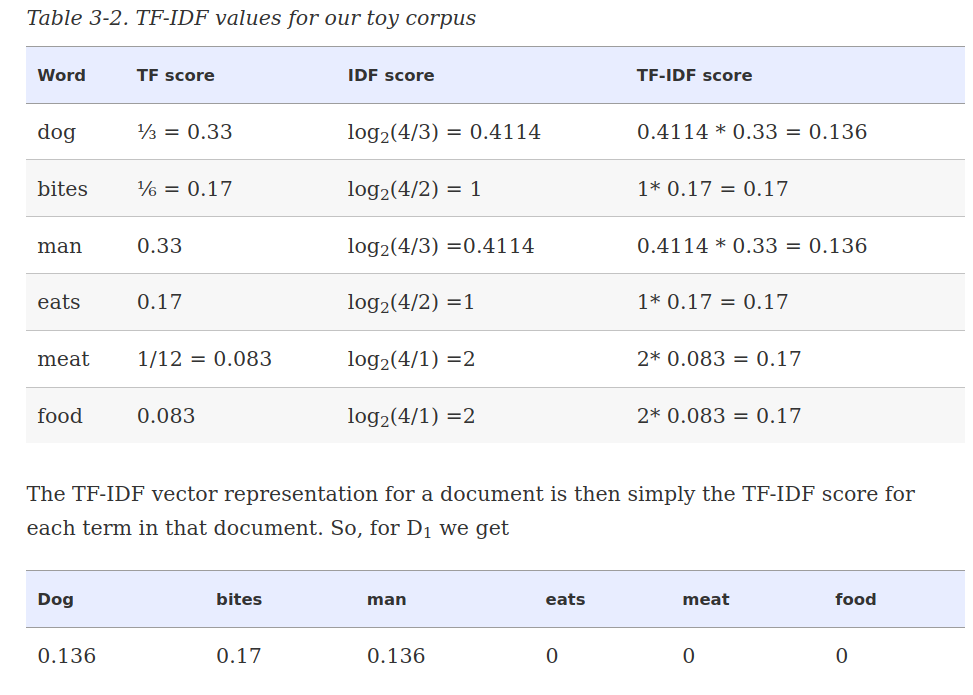
\includegraphics[width=0.9\textwidth]{figures/tfidf.png}
\end{frame}

\begin{frame}[fragile]
\frametitle{TF-IDF code}
\tiny
\begin{verbatim}
from sklearn.feature_extraction.text import TfidfVectorizer

tfidf = TfidfVectorizer()
bow_rep_tfidf = tfidf.fit_transform(processed_docs)
print(tfidf.idf_) #IDF for all words in the vocabulary
print(tfidf.get_feature_names()) #All words in the vocabulary.

temp = tfidf.transform(["dog and man are friends"])
print("Tfidf representation for 'dog and man are friends':\n", temp.toarray())
\end{verbatim}
Note: There are some variations of the formula in practice. 
\end{frame}

\begin{frame}
\frametitle{Pros and Cons of TFIDF}
\begin{itemize}
\item We can use the TF-IDF vectors to calculate similarity between two texts using a similarity measure like Euclidean distance or cosine similarity. 
\item TF-IDF is a commonly used representation in application scenarios such as information retrieval and text classification.  \pause
\item However, despite the fact that TF-IDF is better than the vectorization methods we saw earlier in terms of capturing similarities between words, it still suffers from the curse of high dimensionality. 
\end{itemize}
\end{frame}

\begin{frame}
\frametitle{Embeddings}
Distributionally simliar words are words that are likely to occur in similar contexts.
\begin{itemize}
\item If we’re given the word “USA,” distributionally similar words could be other countries (e.g., Canada, Germany, India, etc.) or cities in the USA. 
\item  If we’re given the word “beautiful,” words that share some relationship with this word (e.g., synonyms, antonyms) could be considered distributionally similar words. 
\end{itemize} \pause
Modern day NLP is based text representations which **learn** such semantic relationships in a dense, low dimensional space (compared to sparse, high dimensional space we saw earlier)
\end{frame}

\begin{frame}[fragile]
\frametitle{Word Embeddings}
\begin{itemize}
\item pre-trained: such embedding representations are already learnt by training on a large database such as wikipedia. We can download the learnt models and directly use them.
\item e.g., word2vec, glove, fastText etc. 
\end{itemize} \tiny
\begin{verbatim}
from gensim.models import Word2Vec, KeyedVectors
pretrainedpath = "NLPBookTut/GoogleNews-vectors-negative300.bin"
w2v_model = KeyedVectors.load_word2vec_format(pretrainedpath
             , binary=True)
print('done loading Word2Vec')
print(len(w2v_model.vocab)) 
#Number of words in the vocabulary.
print(w2v_model.most_similar['beautiful'])
W2v_model['beautiful']
\end{verbatim}
\end{frame}

\begin{frame}
\frametitle{}
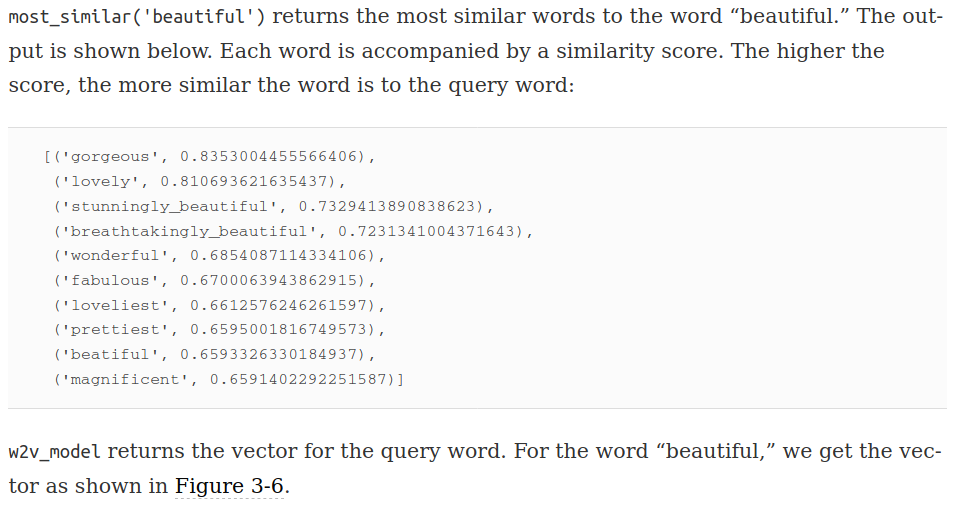
\includegraphics[width=0.9\textwidth]{figures/beautiful.png}
\end{frame}

\begin{frame}[fragile]
\frametitle{Document Embedding}
\begin{itemize}
\item We can obtain the vector representation for an entire text by averaging individual word vectors.
\end{itemize} \tiny
\begin{verbatim}
import spacy
import en_core_web_sm

# Load the spacy model. This takes a few seconds.
nlp = en_core_web_sm.load()

# Process a sentence using the model
doc = nlp("Canada is a large country")

#Get a vector for individual words
#print(doc[0].vector) #vector for 'Canada', the first word 
print(doc.vector) #Averaged vector for the entire sentence
\end{verbatim}
\end{frame}

\begin{frame}
\frametitle{The OOV problem}
\begin{itemize}
\item We can also train our own word embeddings, but both pre-trained and self-trained word embeddings depend on the vocabulary they see in the training data. 
\item What should we do when we encounter a new word in a document? \pause
\item A simple approach that often works is to exclude those words from the feature extraction process so we don’t have to worry about how to get their representations.
\item Another way to deal with the OOV problem for word embeddings is to create vectors that are initialized randomly, where each component is between –0.25 to +0.25, and continue to use these vectors. 
\item There are also other approaches that handle the OOV problem by modifying the training process by bringing in characters and other subword-level linguistic components.
\end{itemize}
\end{frame}

\begin{frame}
\frametitle{Beyond Words: Contextual representations}
\begin{itemize}
\item In all the representations we’ve seen so far, we notice that one word gets one fixed representation. Can this be a problem? 
\item Well, to some extent, yes. Words can mean different things in different contexts. 
\item For example, the sentences “I went to a bank to withdraw money” and “I sat by the river bank and pondered about text representations” both use the word “bank.” However, they mean different things in each sentence. 
\item Well, to some extent, yes. Words can mean different things in different contexts. For example, the sentences “I went to a bank to withdraw money” and “I sat by the river bank and pondered about text representations” both use the word “bank.” However, they mean different things in each sentence. 
\end{itemize}
\end{frame}

\begin{frame}
\frametitle{SOTA: Universal Text Representations}
\begin{itemize}
\item Neural architectures such as recurrent neural networks (RNNs) and transformers were used to develop large-scale models of language (BERT, and beyond), which can be used as pre-trained models to get text representations. 
\item Process: Take a large pre-trained model, and "fine-tune" it to a given task/dataset. 
\item These models have shown significant improvements on some fundamental NLP tasks, such as question answering, semantic role labeling, named entity recognition, and coreference resolution, to name a few. 
\item There are a lot of custom models, especially for BERT, such as: SciBERT, LAWBert, FinBERT, PatentBERT, BioBERT etc.
\end{itemize}
\end{frame}

\begin{frame}[fragile]
\frametitle{An example using BERT}
\tiny
    \begin{verbatim}
        from transformers import AutoTokenizer, AutoModel, pipeline
        modelpath = "bert-base-uncased"
        model = AutoModel.from_pretrained(modelpath, cache_dir=cache_dir)
        tokenizer = AutoTokenizer.from_pretrained(modelpath, cache_dir=cache_dir)
        nlp = pipeline('feature-extraction')
        myrep = nlp(sometext)[0][0]
    \end{verbatim}
    Check examples \href{https://colab.research.google.com/github/mrm8488/shared_colab_notebooks/blob/master/Huggingface_pipelines_demo.ipynb}{here}
\end{frame}

\begin{frame}
\frametitle{Conclusion}
\begin{itemize}
\item we saw different techniques for representing text, starting from the basic approaches to state-of-the-art DL methods. 
\item When should we use what? \pause
\item For some applications, such as text classification, it’s more common to see vectorization approaches and embeddings as the go-to feature representations for text. 
\item For some other applications, such as information extraction, it’s more common to look for handcrafted, domain-specific features. 
\item Quite often, a hybrid approach that combines both kinds of features are used in practice.
\item Having said that, BoW, BoN, TFIDF approaches are a great starting point!
\end{itemize}
\end{frame}

\begin{frame}
\frametitle{Resources}
Jupyter notebooks with code examples showing different ways of representing text: \url{https://github.com/practical-nlp/practical-nlp/tree/master/Ch3}
\end{frame}

\begin{frame}{Assignment 1 Description}
    \begin{itemize}
        \item 15\% of the total grade (for those submitting a term paper), 30\% of the grade (for those submitting without).
\item Question 1: Explore the free trials of NLP service providers or libraries and write a small piece of code that takes a sentence as input and does any one of the following: machine translation, named entity recognition, key phrase extraction, part of speech tagging, relation extraction (again, just write code for any functionality among these!)

\item Question 2: Look for a PDF to text conversion library, write a small piece of code that converts a pdf file you input into plain text.

\item For both these questions, write do own your observations about the tool(s) you used (ease of use, accuracy of the result etc).

\item Submit the assignment as follows: 1 pdf file with the observations, and all the associated code files put into one zip file.
    \end{itemize}
\end{frame}

\begin{frame}{ToDo - before next class}
    \begin{itemize}
        \item Participate in the forum and ask any questions about today's class under "NLP Pipeline" forum. 
        \item Think about where do we usually find corpora? If you want some new kind of corpus, how will you go about looking for it?
        \item Think about what kind of file formats will we encounter when we say "corpora". 
        \item Teams. Think about your teams/paper you chose. If you don't know anyone or can't form a team, message me, I will assign a team for you by Friday.
    \end{itemize}
    We will talk more about data acquisition in the next class.
\end{frame}

\end{document}
